There are many ways to work further with the software we have started on.
The first thing we will propose is to do proper testing and fix the bugs that
will show up. Testing should uncover whether the functionality works as 
intended or not. It should also try to see if the games work as intended.

\begin{wrapfigure}{r}{0.6\textwidth}
	\capstart
	\centering
	\vspace{-10pt}
	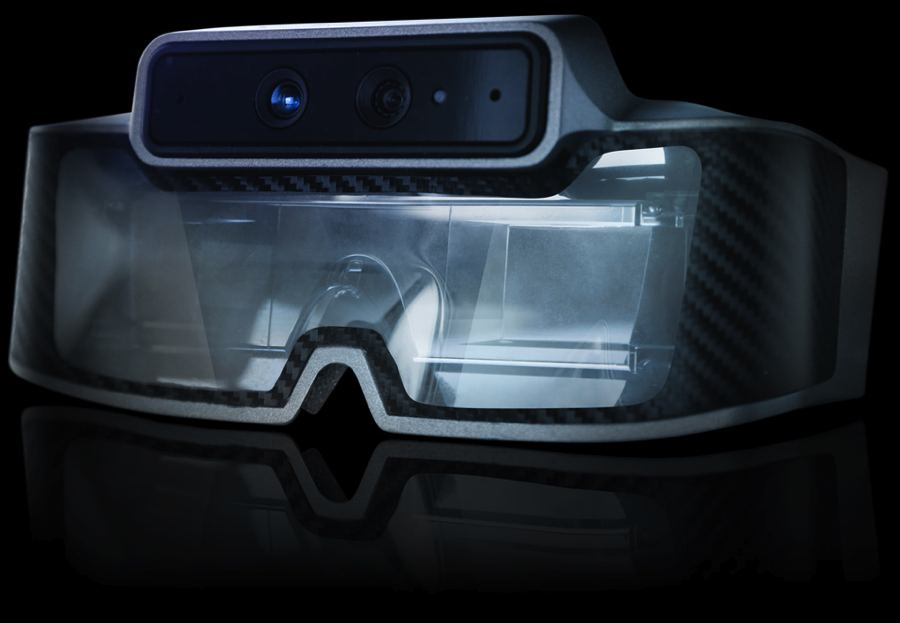
\includegraphics[width=0.58\textwidth]{images/META1_website_image_resized}
	\vspace{-5pt}
	\caption[{META S}paceglasses - Early version]{{META} Spaceglasses. This
	depicts an early version that they sent during a chat conversation on 
	their webpage in January.}
	\vspace{-10pt}
	\label{fig:meta_spaceglasses}
\end{wrapfigure}

One other area that needs to be improved are the graphical user interface (GUI).
It will be a great id\'ea to get professional interaction designers to specify
and create the user interface. The current GUI are responsive to some extent, 
but it have proved not to be good enough. This is highly encouraged to get 
done.

\paragraph{}

When it comes to advancing the software, there are some points we would like 
to mention. One exciting thing to try is to port cogARC to wearable glasses.
Since the original plan was to implement the program for the \gls{Meta 
SpaceGlasses}, these will probably be good to try it on. From their webpage
\cite{MetaSpaceGlasses}, they now, at the 13th of May 2014, claims that new 
orders will start shipping in September. We will expect Kickstarter supporters 
to receive the product a bit before that, so it might be ready to test in only
a few months time if anyone would implement it.

Another advancement is to do something with the tracking and flickering of the 
markers. This is a disturbing factor in the games and would enhance the game
experience if it were fixed. One way is to use an other tracking library than
Vuforia, but there may be tricks that can be done locally to reduce the 
problem. One way can be to handle the input from the library in a more advanced
way.

\paragraph{}

From a more academic perspective, it would be good to look more into the actual
research value of cogARC. When looking at it from that angle, there may show up
several ways to enhance the software. Logging may change in what data that are
being logged and how the data is filtered, stored and used.

New games may be added to investigate in other cognitive functionalities than 
those that are already there. Some of the games that are implemented may be
filtered out, while others may change if they does not serve their purpose well.
